\documentclass[a4paper,journal]{IEEEtran}
\usepackage{amsmath,amsfonts}
\usepackage{algorithmic}
\usepackage{algorithm}
\usepackage{array}
\usepackage[caption=false,font=normalsize,labelfont=sf,textfont=sf]{subfig}
\usepackage{textcomp}
\usepackage{stfloats}
\usepackage{url}
\usepackage{hyperref}
\usepackage{verbatim}
\usepackage{graphicx}
%\usepackage{cite}
\usepackage[numbers]{natbib}
\hyphenation{op-tical net-works semi-conduc-tor IEEE-Xplore}
% updated with editorial comments 8/9/2021

%%%%%%%%%%%%%%%%%%%%%%%%%%%%%%%%%%%%%%%%%%%%%%%%%%%%%%%
% URL line breaks in references
\def\UrlBreaks{\do\/\do-}

% todos
\usepackage{xcolor}
\newcommand{\todo}[1]{\textcolor{red}{TODO: #1}\PackageWarning{TODO:}{#1!}}
%%%%%%%%%%%%%%%%%%%%%%%%%%%%%%%%%%%%%%%%%%%%%%%%%%%%%%%

\begin{document}
	
	\title{Extended Metrics Project for Apache Airflow}%Monitoring of Scientific Workflows
	
	
	
	\author{Julian Legler, Marcin Ozimirski, Matthias Seiler
		% <-this % stops a space
		\thanks{This paper was produced by students of the Technische Universität Berlin in the course ''Master Project: Distributed Systems'' in summer 2022. All results are available in the GitHub repository: \url{https://github.com/maseiler/swms-monitoring}}% <-this % stops a space
		%\thanks{Manuscript received April 19, 2021; revised August 16, 2021.}
	}
	
	% The paper headers
	\markboth{PJ DS - Extended Metrics Project for Apache Airflow}%
	{Shell \MakeLowercase{\textit{et al.}}: A Sample Article Using IEEEtran.cls for IEEE Journals}
	
	%\IEEEpubid{0000--0000/00\$00.00~\copyright~2021 IEEE}
	
	\maketitle
	
	\begin{abstract}
		
		The emergence of Scientific Workflow Management Systems (SWMS) allowed speeding up scientific progress in various fields. The main task of such systems is to represent and manage complex distributed scientific computations. They are designed to handle datasets and examine them in a programmatical way. The software can process given jobs effectively and provide results in a requested form. However, nowadays' scientific calculations can involve hundreds of stages, each integrating several models and data sources created by various research groups. Because of their complexity, they require a significant amount of computing resources to be processed. Such projects are well suited to a cloud environment since it allows for scalability in the event of increased resource demand. In these situations, system monitoring software is essential because it provides a better understanding of how resources are utilized when consecutive tasks are being executed. It can help to decrease the costs by choosing the best suitable provider or adjusting parts of the code for a faster execution time. Unfortunately, the built-in monitoring features offered by the SWMS developers and cloud providers deliver only high-level metrics, such as CPU usage per task, which is not always enough for a detailed resource usage analysis. Therefore the implementation of software allowing for monitoring on a system process level stays on the shoulders of the end users. 
		
		% TODO: state our solution and result
		
	\end{abstract}
	
	\begin{IEEEkeywords}
		Scientific Workflow Management Systems, Monitoring, eBPF
	\end{IEEEkeywords}
	
	%%%%%%%%%%%%%%%%%%%%%%
	% Introduction
	%%%%%%%%%%%%%%%%%%%%%%
	
	\section{Introduction}
	A scientific workflow management system (SWMS) is a commonly used software solution in the field of computational science. It can execute a series of calculations to examine (big) data sets in a structured and organized manner. Such computations are commonly called workflows consisting of tasks related to one another. The Management System is responsible for a transparent orchestration and execution of specified tasks, considering dependencies between them. The software allows for an efficient way to process and extract information from the examined data sets, leading to scientific advances in various fields such as biology, physics, and astronomy\cite{gil2007examiningchallengesscientific}. Yet, such workflows are often resource-intensive and require a distributed, dynamic, and scalable architecture to achieve meaningful results in a reasonable amount of time. The cloud and containerization paradigms offer several advantages when deploying these systems, such as accessibility, flexibility, and scalability \todo{source?}, which allow workflows to be deployed and executed dynamically. These characteristics are crucial, since a with a changing workflow during execution also comes different requirements regarding resources. This could for example depend on an input data set, the parallelism of computed tasks, and their level of complexity. The available resource pool can scale to adjust the computing resources throughout the workflow execution process. However, depending on the technological solutions offered by cloud services, hardware and software factors can vary significantly from one provider to another, which leads to different processing speeds, resource utilization, and error ratio\cite{aljamal2018comparativereviewhighperformance}. Built-in monitoring features provide information on the amount of time and resources needed for the computation of a particular task or resource utilization on the active virtual machines (containers). Unfortunately, for more intense calculations, like machine learning, data delivered by the built-in tools are often insufficient to provide enough information for deep analysis and detection of bottlenecks or finding opportunities for code optimization. In such scenarios, the more detailed (low-level) metrics available, the better conclusions can be drawn regarding the performance of the current solution. Producing exact information on the number of I/O operations, CPU load, or memory usage per system process allows for a more accurate analysis of executed workflows (or their tasks) and the infrastructure on which the calculations are performed. This would open doors for improving of the system architecture, hardware and code. However, the implementation of solutions capable of gathering such information or the extension of the already existing ones rests on the shoulders of the end users. This project intends to provide a solution allowing the collection of high- and low-level metrics, independently of underlying cloud technology and SWMS used for computational science. The following report is structured as follows \todo{}
	
	%%%%%%%%%%%%%%%%%%%%%%
	% Related Work
	%%%%%%%%%%%%%%%%%%%%%%
	
	\section{Related Work}
	% TODO: previous research on SWMS, eBPF
	Due to the nature of high volume data, modern science is often conducted on high-performance computing infrastructures. In recent years, the complexity of both scientific experiments, as well as that of its underlying infrastructure has grown tremendously, reaching the point where it becomes challenging to execute the workflows in a reliable and error-free way. On the scale at which such projects are carried out it is almost certain that software or infrastructure anomalies will occur, which makes the detection and diagnosis of system failures more challenging than ever before. In order to address such issues, \citeauthor{valerio2008capturingworkflowevent} created a prototype system monitoring the following \todo{} properties at any time during and after the execution of the workflow. The premise of the design is to enable the user to answer the following questions:
	
	\begin{itemize}
		\item What is the status of the workflow?
		\item Did the user make changes to the workflow before executing it?
		\item Why did it fail at a certain point?
		\item What was the execution context of the workflow directly before it failed?
		\item How many resources does it consume?
		\item How has each activity in the workflow performed (in the past)?
	\end{itemize}
	
	The ability to answer the aforementioned questions can be guaranteed by a system monitoring the general properties of the workflow and its slightest details. Therefore, this type of solution usually consists of various components that collect data at different layers, starting from the general parameters of the workflow through the infrastructure on which it is run, ending with individual processes responsible for performing calculations. In addition, the software must be able to map the relevant processes (which can be executed in a parallel and distributed manner) to the corresponding machines and tasks and publish them in a readable form. Of course, all this makes sense only if one can assign a chronological order of these processes concerning the time domain. Furthermore, an environment in which such scenarios are executed also plays an important role. Regardless of whether the code is invoked in the operating system context or a virtualized container created for the task, it is often characterized by restrictive standards. Such standards fulfill the functions of stability and security and thus may not provide any or only limited opportunities for adjustment. However, without it, it may not be possible to access system values available to the system's kernel. 
	Fortunately, one does not have to develop everything from scratch as there are open technologies capable of solving a single or part of the listed conditions. \citeauthor{levin2020viperproberethinkingmicroservice} used Linux’s extended Berkeley Packet Filter (eBPF)\cite{ebpf} software for a collection of system metrics in the containerized environment and exposure of these to a specified endpoint. In a further step, he used Grafana\cite{grafana}, an observability framework, to present the collected information using programmable dashboards. This strategy allows the collection of data from various sources and then processing and presenting it in the form of histograms and graphs, as described by the user. It also reflects well the current trend for creating monitoring solutions. It is based on a combination of available platforms and software to collect and present data that are relevant to a carried-out project. For such approaches, it is not important what generates or where the data comes from, as long as it is published in a suitable format, which is most often JSON or some derivative of XML.
	
	%%%%%%%%%%%%%%%%%%%%%%
	% Background
	%%%%%%%%%%%%%%%%%%%%%%
	
	\section{Background}
	% TODO: describe technologies we are using
	% SWMS, Airflow
	Today exists a vast number of workflow management systems, ranging form general purpose ones like Apache Airflow \cite{airflow}, Nextflow \cite{nextflow} or Pegasus \cite{pegasus} to domain specific ones e.g. Taverna \cite{taverna} for bio-informatics and astronomy, Arvados \cite{arvados} for biomedical data, and many more. Each of these naturally have their advantages and disadvantages over another, due to their design and architecture and thus resulting in different stages of maturity.\\
	To begin with, we decided for Airflow, since it serves the general purpose, is widely used and one of the most mature SWMS \cite{harenslak2021data}. The workflow in Airflow is described with a Directed Acyclic Graph (DAG), whose nodes consists of tasks that are executed. The edges represent the dependencies and therefore the execution order of these tasks. The description of the DAG is specified by the user in a Python script. Figure \ref{fig:aiflow:dag} shows a DAG that runs tests in a Kubernetes environment \cite{airflowDag}.
	\begin{figure*}[h]
		\centering
		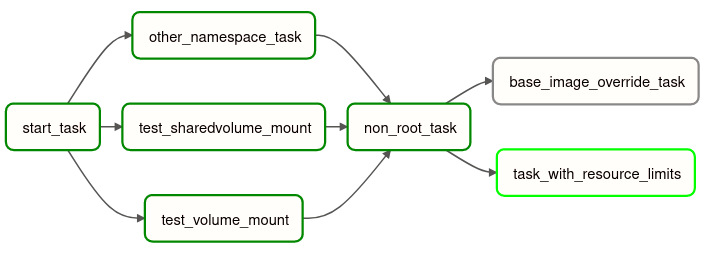
\includegraphics[width=0.7\linewidth]{images/airflow-dag.png}
		\caption{Airflow DAG with five tasks successfully run (dark green), one running (light green) and one in queue (gray). The execution order is defined by the connections between the individual tasks. After the \textit{start\_task} task is finished, the connected tasks can start in parallel. Afterwards, the task \textit{non\_root\_task} has to wait until \textit{other\_namespace\_task}, \textit{test\_sharedvolume\_mount} and \textit{test\_volume\_mount} has successfully finished before it can get executed.}
		\label{fig:aiflow:dag}
	\end{figure*}
	
	As depicted in Figure \ref{fig:aiflow:arch}, the basic architecture of Airflow consists of the following components: the \textit{User Interface} (UI), that is served by the \textit{Webserver}, is the entry point for the user, and not only feature-rich, but also easy to use. At the heart of Airflow resides the \textit{Scheduler}, ''which handles both triggering scheduled workflows, and submitting Tasks''\cite{airflowArchitecture}. It therefore requires access to a \textit{DAG Directory}, in order to makes use of one of the provided \textit{Executor}s \cite{airflowExecutor}, that handle these tasks. The actual execution of tasks is performed by one or more \textit{Workers}. Finally, a \textit{Metadata Database} is ''used by the scheduler, executor and webserver to store state''\cite{airflowArchitecture}.
	\begin{figure}[h]
		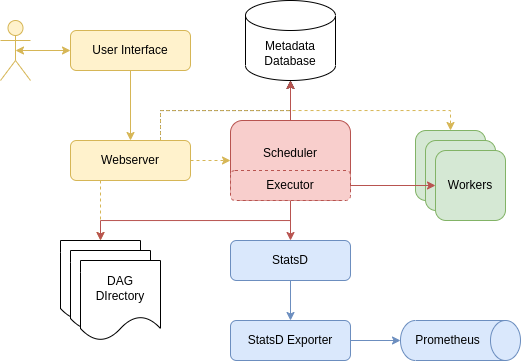
\includegraphics[width=\linewidth]{images/airflow-architecture.png}
		\caption{Airflow architecture}
		\label{fig:aiflow:arch}
	\end{figure}
	
	Airflow provides built-in logging and monitoring \cite{airflowMonitoring}, whose monitoring stack relies on StatsD \cite{statsd}, that gathers the internal metrics and exposes them to Prometheus. StatsD creates buckets and fills them with values for the specific metric, that will be aggregated after a predefined period and flushed to an endpoint for further processing. While the are numerous metrics on DAG and task level, none of them consider metrics on lower levels \cite{airflowMetrics}.
	
	% Monitoring, eBPF
	With eBPF \cite{ebpf} however, it is possible to gather metrics directly from the Linux kernel. It extends the kernel without changing the kernel source code or loading kernel modules and has therefore unrestricted access to all hardware. These little programs get triggered by certain hook point (e.g. system calls, function entry/exit, network events) and can thus be attached to almost anywhere into kernel or user applications \cite{whatebpf}. eBPF programs are usually written using frameworks such as the BPF Compiler Collection (BCC) \cite{bcc}. BCC provides a library and ''Python, C\texttt{++}, and Lua interfaces for writing programs''\cite{cassagnes2020riseebpfnonintrusive} and many tools for efficient kernel tracing.
	Figure \ref{fig:ebpf:steps} depicts the involved steps to attach an eBPF program: in order to use the program in the Linux kernel, it expects the program in the form of bytecode. With the \texttt{bpf} system call, the program will be loaded into kernel space, where it first has to be verified (that is actually safe to run) and secondly compiled to machine specific instructions. ''This makes eBPF programs run as efficiently as natively compiled kernel code or as code loaded as a kernel module'' \cite{whatebpf}.
	\begin{figure}[h]
		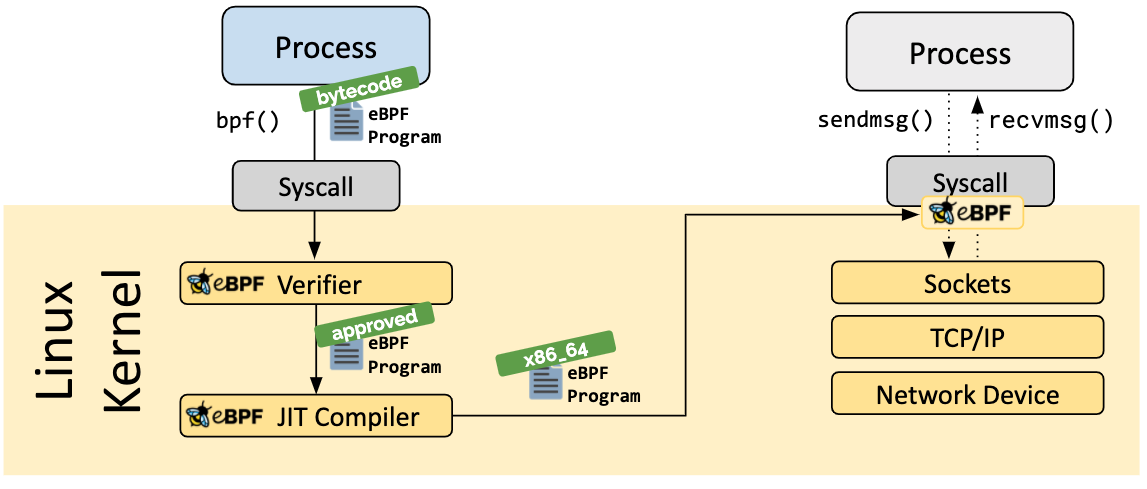
\includegraphics[width=\linewidth]{images/ebpf-steps.png}
		\caption{Steps to attach an eBPF program \cite{whatebpf}}
		\label{fig:ebpf:steps}
	\end{figure}
	In order to store collected information (e.g. in the form of metrics), eBPF leverages \textit{eBPF Maps} \cite{ebpfMaps}, that can be accessed not only from kernel, but also from user space.
	
	% Monitoring, Prometheus, Grafana
	The data from these eBPF maps can be exported to a more powerful monitoring systems such as Prometheus, Graphite or InfluxDB, and  visualized with an analytics platform like Grafana or Kibana.
	
	%%%%%%%%%%%%%%%%%%%%%%
	% Approach
	%%%%%%%%%%%%%%%%%%%%%%
	
	\section{Approach}
	% TODO: how we implemented tech mentioned in background
	As mentioned in the previous section, we are going to build the monitoring solution on top of the Scientific Workflow Management System (SWMS) Apache Airflow. 
	
	\subsection{Deployment of Apache Airflow}
	Apache Airflow is a widely used and adopted SWMS and as such, there are many approaches for deployment. These include fully managed solutions like Google Cloud Composer, Amazon Managed Workflows for Apache Airflow and astronomer.io. Using such services comes with the advantage of an easy and fast deployment. The downside is, that you may lack some flexibility and access to more granular and in depth functionalities and access to all resources. An Airflow instance deployed by such services can often just be treated as a black box system. This approach may block some needed functionalities and access to the raw resources required to collect metrics at the level of granularity we try to achieve.
	
	On the other side of the deployment complexity are the deployment strategies that involves deploying or sometimes even compiling the needed components yourself on bare-metal servers. For this, the database and logging systems have to be correctly installed beforehand. At the same time, machines have to be configured to build a cluster and then Apache Airflow is installed and run on all the machines. This could also be combined by deploying Kubernetes in the first place, and then using Kubernetes orchestration technologies to run all the needed services in the cluster. This deployment strategy comes with the advantage of fine and granular access to all system resources, and the downside of the overhead when managing everything by oneself. 
	
	%On the other end of the deployment complexity spectrum are deployment strategies that involve deploying or even compiling the required components on bare-metal servers. This requires that the database and logging systems be properly installed beforehand. At the same time, machines must be configured to form a cluster, and Apache Airflow must be installed and run on all of them. This could also be combined by first deploying Kubernetes and then using Kubernetes orchestration technologies to run all of the necessary services in the cluster. This deployment strategy has the advantage of fine and granular access to all system resources, but the disadvantage of the overhead associated with managing everything oneself.
	
	A deployment strategy is picked, that combines the two above. Google Cloud Platform (GCP) is used as the provider for the needed computation power provided by their different cloud services. GCP provides managed resources and guarantees an easy-to-use process of deploying the needed infrastructure. With the Google Kubernetes Engine (GKE) it even provides a managed Kubernetes deployment. Using this, the services no longer have to be installed on the individual machines, they can rather be just send to Kubernetes, which then orchestrates the needed services and deploy them on the available infrastructure. At the same time, one has full access to all the underlying components, like the virtual machines Kubernetes and the Apache Airflow services running on. This combines the granular access to all resources, and the ease of using a managed service.
	
	GKE is configured to create three nodes of the type e2-standard-4 which consist of 4 vCPUs and 16 GB RAM. \cite{gcpMachineType}
	For the deployment of Apache Airflow on top of Kubernetes the official Apache Airflow Helm Chart is used. \cite{airflowHelmChart} Using a Helm Chart is a good way to reduce further complexity by using a pre-defined, out of the box running, Apache Airflow configuration. 
	
	The original Helm Chart \cite{airflowHelmChart} was altered in the following ways to deal with our requirements.
	\subsubsection{Executor}
	
	\begin{figure*}[h]
		\centering
		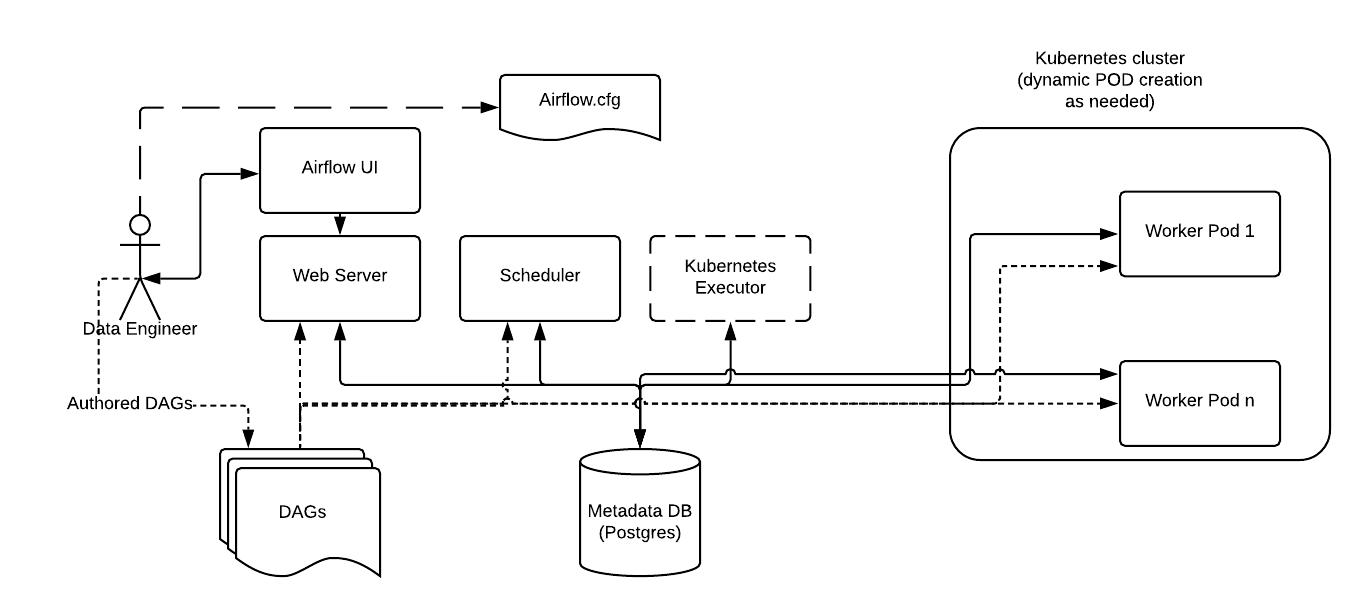
\includegraphics[width=0.9\linewidth]{images/arch-diag-kubernetes.png}
		\caption{Overview of the architecture when using the Kubernetes Executor. Showing the services and possible interaction by a user. Every task is run on an newly created worker pod that is permanently destroyed when the job has finished. The graphic is lacking the metric and logging part of Airflow which is shown in \autoref{fig:aiflow:arch}. The graphic is from \cite{airflowExecutorKubernetes}}
		\label{fig:airflow_arch_kubernetes}
	\end{figure*}
	
	There are different Apache Airflow Executors with different approaches on how to handle the execution of tasks. It would make sense to use the default Celery Executor or the Kubernetes Executor for this project. The Celery Executor is adding a queue to the deployment. On all available nodes, a worker will be deployed. The workers continuously fetch new jobs from the queue and execute them.  The Kubernetes Executor, on the other hand, is changing the behavior in the way, that each node does not have only one worker, but rather for each job there is one worker which is terminated when the job is finished. The huge advantage of the Kubernetes Executor is, that this executor is using the labeling capabilities of Kubernetes. The Kubernetes Executor is very communicative in the worker name and metadata, which makes it easy to collect all this information without accessing the machine. \cite{airflowExecutor}\cite{airflowExecutorKubernetes} The following data is attached to every worker pod when using the Kubernetes Executor:
	\begin{itemize}
		\item dag\_id, which is the name of the executed DAG. This name is not unique but helps with identifying the context.
		\item run\_id, which is an timestamp and a unique id that is assigned when triggering the DAG.
		\item task\_id, which is the name of the executed task in this worker pod. This name is also not unique but is an important information on what is currently running inside this pod for later analyses.
	\end{itemize}
	
	With the help of these information we can reliably identify the current task, the containing DAG and the corresponding triggered run instance of the DAG. All these information are crucial for the further work. Without knowing whats inside the pods, a lot of valuable information would get lost. Luckily all these information are supplied simply by using the Kubernetes Executor. Alternative strategies would probably include writing own code to detect the running processes on the pods and then mapping them via the Airflow API to the corresponding DAG and run. Work in this direction was done in the beginning, but was eventually abandoned because of the advantages offered by the Kubernetes Exporter.
	
	\subsubsection{StatsD}
	StatsD is the monitoring service used by Apache Airflow. To get the metrics compatible to Prometheus, a mapping is configured so that the values can get interpreted correctly by Prometheus. The StatsD Exporter is shipped with the used official Helm Chart for Apache Airflow.
	
	\subsubsection{Webserver, Worker, Environment}
	Here are just minor changes, so that the webserver can be accessed easily for executing test DAGs, Apache Airflow knows the exact number of nodes the executor can use, and the environment parameters are changed to enable the backend authentication mechanism for accessing the Apache Airflow API and deploying Apache Airflow with the sample DAGs for better demonstration. 
	
	\subsubsection{Prometheus and Grafana}
	
	For our monitoring stack, we rely on Prometheus and Grafana, which we had to adjust to our new needs:
	
	\begin{itemize}
		\item Apache Airflows StatsD Exporter is added as a scraping target. Prometheus now collects every 15 seconds the mapped metrics collected by StatsD
		\item Every Endpoint orchestrated by Kubernetes is scraped every 5 seconds to collect the values collected by the eBPF Exporter
	\end{itemize}
	
	The kube-state-metrics service is configured to send all labels and annotations from all pods in all namespaces and not stripping them away before sending them to Prometheus, which is the default behaviour and can lead to confusion.
	
	Because of the mapping already done via the StatsD exporter, the metrics are parsable and interpretable as normal Prometheus metrics and can be used like normal metrics to create custom Grafana dashboards. A few possible examples of metrics and how to visualize them are demonstrated in \autoref{sec:results}.
	
	\subsection{eBPF Exporter}
	Since we use Prometheus for metric gathering, we need an exporter that is able to publish the eBPF metrics. Developers at Cloudflare created an \textit{ebpf\_exporter} \cite{ebpfCloudflare} that does exactly this. However, we had to adjust the exporter \cite{ebpfExporterJulian}, so that we can retrieve the airflow labels DAG ID, Task ID and Run ID. For this a previously unaccepted pull request from the Cloudflare project was used as an example on how to use eBPF to get information form Kubernetes \cite{ebpfPull75}. This pull requests contain an example implementation for exporting the eBPF metrics using also information provided by Kubernetes about the containing node or pod. The implementation was used as a starting point, but had to be completely re implemented as they used the dockerd implementation and therefore the Docker API which is no longer supported in newer Kubernetes versions \cite{kubernetesDockerDepricated}. Because of the lack of documentation for the now used containerd API, the code was rewritten to use the Kubernetes API. This introduces new problems, because now one also has to deal with authentication mechanics as the Kubernetes API can manage the whole cluster and has no internal pod specific permissions for just getting information on ourselves. To tackle this, a cluster role binding with the needed permissions is used as suggested by \cite{kubernetesRbac}. With this changes finally the DAG ID, Task ID and Run ID where published by the eBPF exporter together with the selected metrics.
	
	These parameters can be used to filter the results in Grafana.
	
	To make the deployment as easy as possible, we created a Helm chart using a Docker image, where one can supply a configmap with eBPF programs. Per default we provide five examples \cite{ebpfexporterexamples}:
	\begin{itemize}
		\item \textit{biolatency}~ traces the block device I/O (disk I/O), and records the distribution of I/O latency,
		\item \textit{cachestat}~ records page cache accesses,
		\item \textit{dcstat}~ exposes statistics on the Linux  directory  entry cache,
		\item \textit{runqlat}~ monitors how long tasks spent waiting their turn to run on-CPU, and
		\item \textit{syscalls}~ measures the latency of syscalls, including the entrypoint and audit logging.
	\end{itemize}
	
	The configmap can be easily extendable with additional eBPF programs.
	
	%%%%%%%%%%%%%%%%%%%%%%
	% Results
	%%%%%%%%%%%%%%%%%%%%%%
	
	\section{Results}
	\label{sec:results}
	In the following we will show some results of our system, when we executed the DAG \textit{example\_complex } provided by Airflow \cite{exampleComplex} on three worker nodes. This workflow was executed around 11:36:30 and completed within 2:50 minutes.
	
	As we can see by the colors in Figure \ref{fig:results:runqlat:a}, there is increased activity between 11:37:00 and 11:39:00, with a peak (red square) where over 5700 CPU tasks had to wait between 8 µs and 16.00 µs before they could be processed by the CPU.
	The same behaviour can be observed in Figure \ref{fig:results:runqlat:b}, which shows that the average waiting time is around 185 µs and the maximum 90th and 95th percentile at 243 µs and 1.58 ms respectively.
	\begin{figure}[h]
		\begin{subfigure}
			\centering
			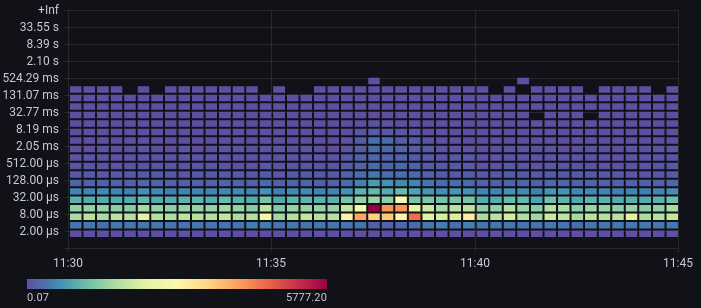
\includegraphics[width=\linewidth]{images/results_runqlat_latency.png}
			\caption{Heatmap of run queue latency of a single node.}
			\label{fig:results:runqlat:a}
		\end{subfigure}
		\hfill
		\begin{subfigure}
			\centering
			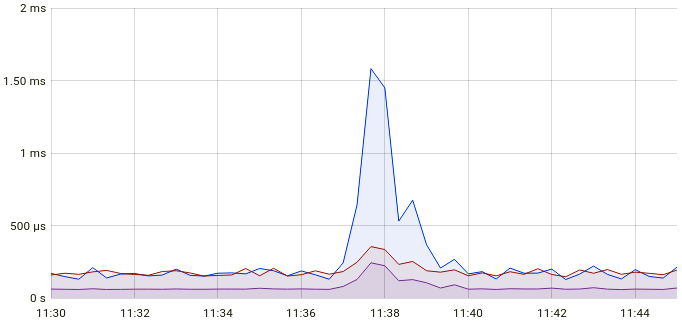
\includegraphics[width=\linewidth]{images/results_runqlat_percentile.png}
			\caption{Average (blue), 95th percentile (green) and 90th percentile (green) of run queue latency on a single node.}
			\label{fig:results:runqlat:b}
		\end{subfigure}
	\end{figure}
	
	In regard to system calls, we can see in Figure \ref{fig:results:syscalls}, that \texttt{do\_syscall\_64}, which was instructed from user space to perform a system call, had higher latencies before the DAG was triggered.
	\begin{figure}[h]
		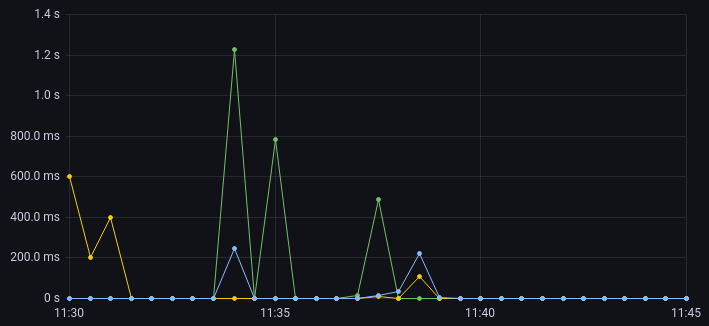
\includegraphics[width=\linewidth]{images/results_syscalls_total.png}
		\caption{System call latency for three worker nodes.}
		\label{fig:results:syscalls}
	\end{figure}
	
	The cache statistics are unfortunately not very meaningful, presumably because the exporter could not keep up with larger spikes of data. Nonetheless, one can observe in Figure \ref{fig:results:cachestat} that there has been a large increase in cache reads during workflow execution.
	\begin{figure}[h]
		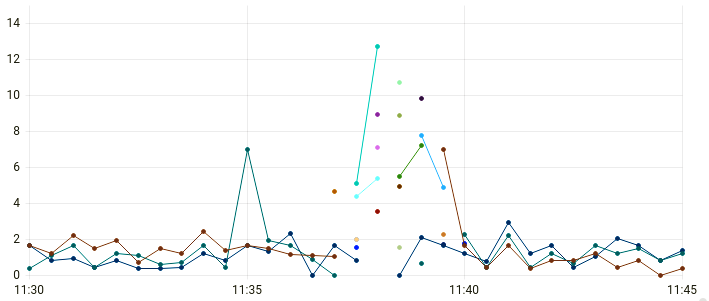
\includegraphics[width=\linewidth]{images/results_cachestat_access.png}
		\caption{Cache reads for three worker nodes.}
		\label{fig:results:cachestat}
	\end{figure}
	
	\section{Discussion}
	% TODO: results and challenges
	While our five examples demonstrate that it is possible to extend metrics for SWMS using eBPF, it does not fulfill the scope we imagined.
	% eBPF issue
	First, eBPF strongly depends on the underlying hardware and its access through the virtualization layer. Unfortunately, GCP does not allow access to certain \texttt{perf} events (e.g. CPU cycles, CPU instructions, cache misses, ...), limiting the number of available programs quite significantly. This issue pertains also other virtualization solutions \cite{ebpfVirtIssue1}\cite{ebpfVirtIssue2}\cite{ebpfVirtIssue3}. We assume, that this issue does not occur on bare-metal hardware, but were not able to verify this hypothesis yet.
	
	% other SWMS issue
	Secondly, \todo{@Marcin Nextflow}
	
	\subsection{Future Work}
	As stated in previous chapters, we were able to demonstrate a proof of concept, that could become relevant in industry, if the above issues were solved. Our solution with BCC has manifold opportunities to gather more system information. On top of that, one could integrate bpftrace as an alternative to BCC, to get an even richer set of eBPF programs. 
	In order to deploy our monitoring solution to other cloud providers (e.g. AWS, Azure), other setup scripts are needed. Due to the above mentioned issue, a solution for bare-metal machines using k3s \cite{k3s} would be extremely valuable. 
	More than that, other SWMS should be supported to attract a wide range of users and developers. Making the metrics loosely coupled is a crucial step hereby.
	Ultimately, a small benchmark suite would be very helpful to evaluate the overhead of the eBPF exporter on the overall system performance.
	
	%%%%%%%%%%%%%%%%%%%%%%
	% Conclusion
	%%%%%%%%%%%%%%%%%%%%%%
	
	\section{Conclusion}
	\todo{}
	
	\section*{Acknowledgments}
	We thank our supervisor Sören Becker for his enormous support and patience. 
	
	% References
	\bibliography{bib}
	\bibliographystyle{IEEEtranN}
	
\end{document}